\section{Risultati}

Per dimostrare la scalabilità orizzontale dell'applicazione sono state utilizzate le seguenti
macchine:

\begin{enumerate}
    \item un laptop con Intel core i5 e 8gb ram,
    \item un laptop con Intel core i7 e 16gb ram
\end{enumerate}

La maggior parte dei servizi necessari all'applicazione sono stati eseguiti sulla prima macchina:
TimescaleDB, Kafka, i producer, l'istanza master di Spark, alcune istanze worker ed
infine il processo submit di Spark che avvia l'esecuzione della StreamApp all'interno del cluster.

Nella seconda macchina sono stati eseguiti soltanto Spark workers appartenenti allo stesso cluster.

Ogni worker dispone di 1 cpu e 1gb di ram ed il loro numero è stato incrementato gradualmente
allo scopo di testare la scalabilità dell'applicazione in questo modo:

\begin{itemize}
    \item inizialmente (alle 20:50 circa) è stato eseguito un solo worker nella prima macchina
    \item tre minuti dopo ne è stata eseguita un'altra istanza sulla prima macchina
    \item d'ora in poi ogni 3 minuti è stato aggiunto un worker sulla seconda macchina fino a
          a raggiungere un totale di 10 worker sulla seconda macchina più 2 sulla prima
    \item infine sono stati aggiunti altri 4 worker sulla seconda macchina sempre ad intervalli di
          tre minuti.
\end{itemize}

\begin{center}
    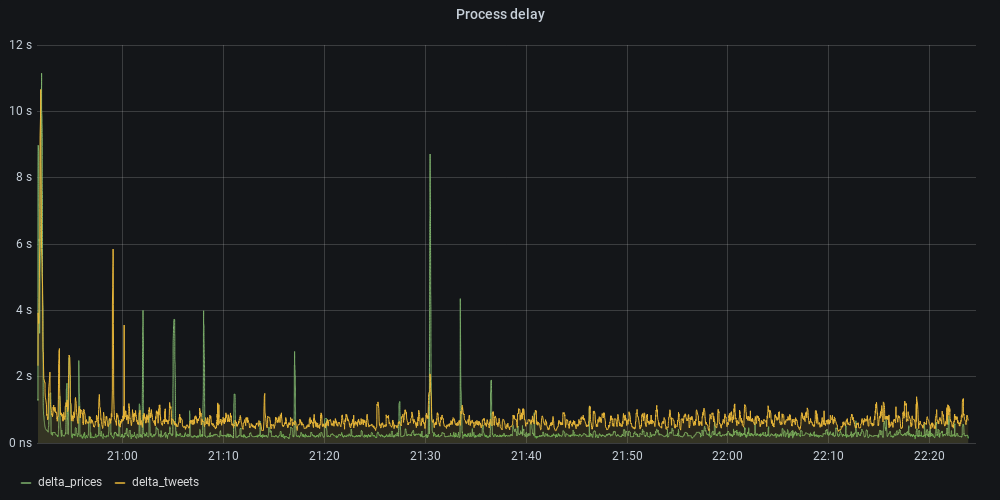
\includegraphics[max width=\linewidth]{process_delay.png}
    \captionof{figure}{Ritardo tra ricezione ed elaborazione dei dati ricevuti}
    \label{processdelay}
\end{center}


Nella Figura \ref{processdelay} è riportato il grafico che mostra il ritardo nell'analisi dei tweets
(in giallo) e dei prezzi (in verde) ricevuti calcolato come differenza tra il momento di ricezione
(aggiunto dai producer) ed il momento subito precedente all'inserimento nel database.

Si può notare che generalmente i tempi richiesti (mediamente 300ms per i prezzi e 750ms per
i tweets) siano pressoché indipendenti dal numero di worker,
probabilmente significando che uno o due worker sono in grado di gestire il flusso medio di dati
ricevuto (mostrato in Figura \ref{rate}).
Ed è altrattando evidente come all'aumentare del numero dei worker diminuiscano numero e 
frequenza dei "picchi" probabilmente dovuti alle oscillazioni nella frequenza dei messaggi ricevuti.

\begin{center}
    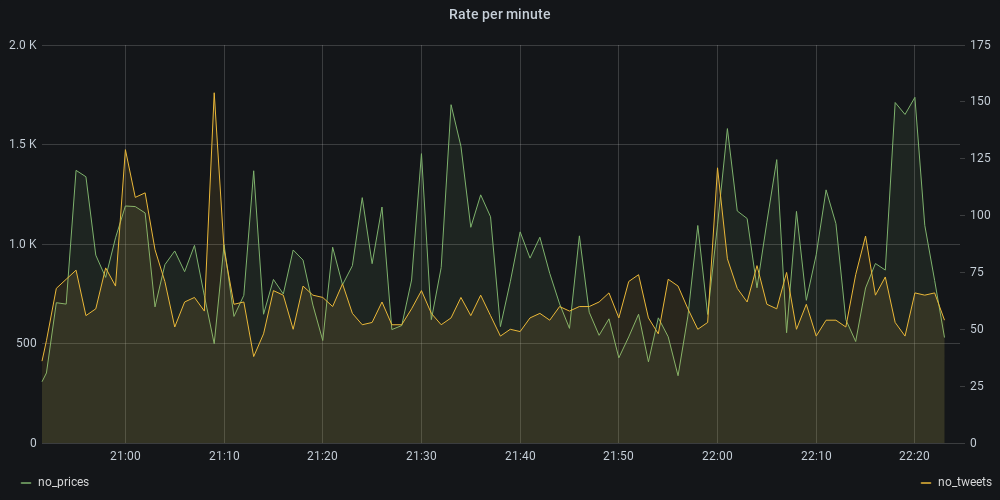
\includegraphics[max width=\linewidth]{rate.png}
    \captionof{figure}{Numero di messaggi ricevuti al minuto}
    \label{rate}
\end{center}

In Figura \ref{rate} è riportato il numero di messaggi ricevuti al minuto da Twitter, in giallo
sull'asse delle ordinate destro, e da Binance, in verde sulle ordinate a sinistra, nell'intervallo
di tempo preso in analisi.
Riassumendo sono stati ricevuti ogni minuto in media 895 messaggi relativi ai prezzi con un
massimo di 1737, mentre per quanto riguarda i tweets mediamente 64 con un massimo di 154. 

